\documentclass{standalone}
\usepackage{tikz}
\usetikzlibrary{patterns}
\usetikzlibrary{positioning}
\usetikzlibrary{patterns, positioning}
\usetikzlibrary{shapes.misc}
\usepackage[outline]{contour}
\contourlength{1.5pt} 
\usepackage[sfdefault]{ClearSans}

\begin{document}
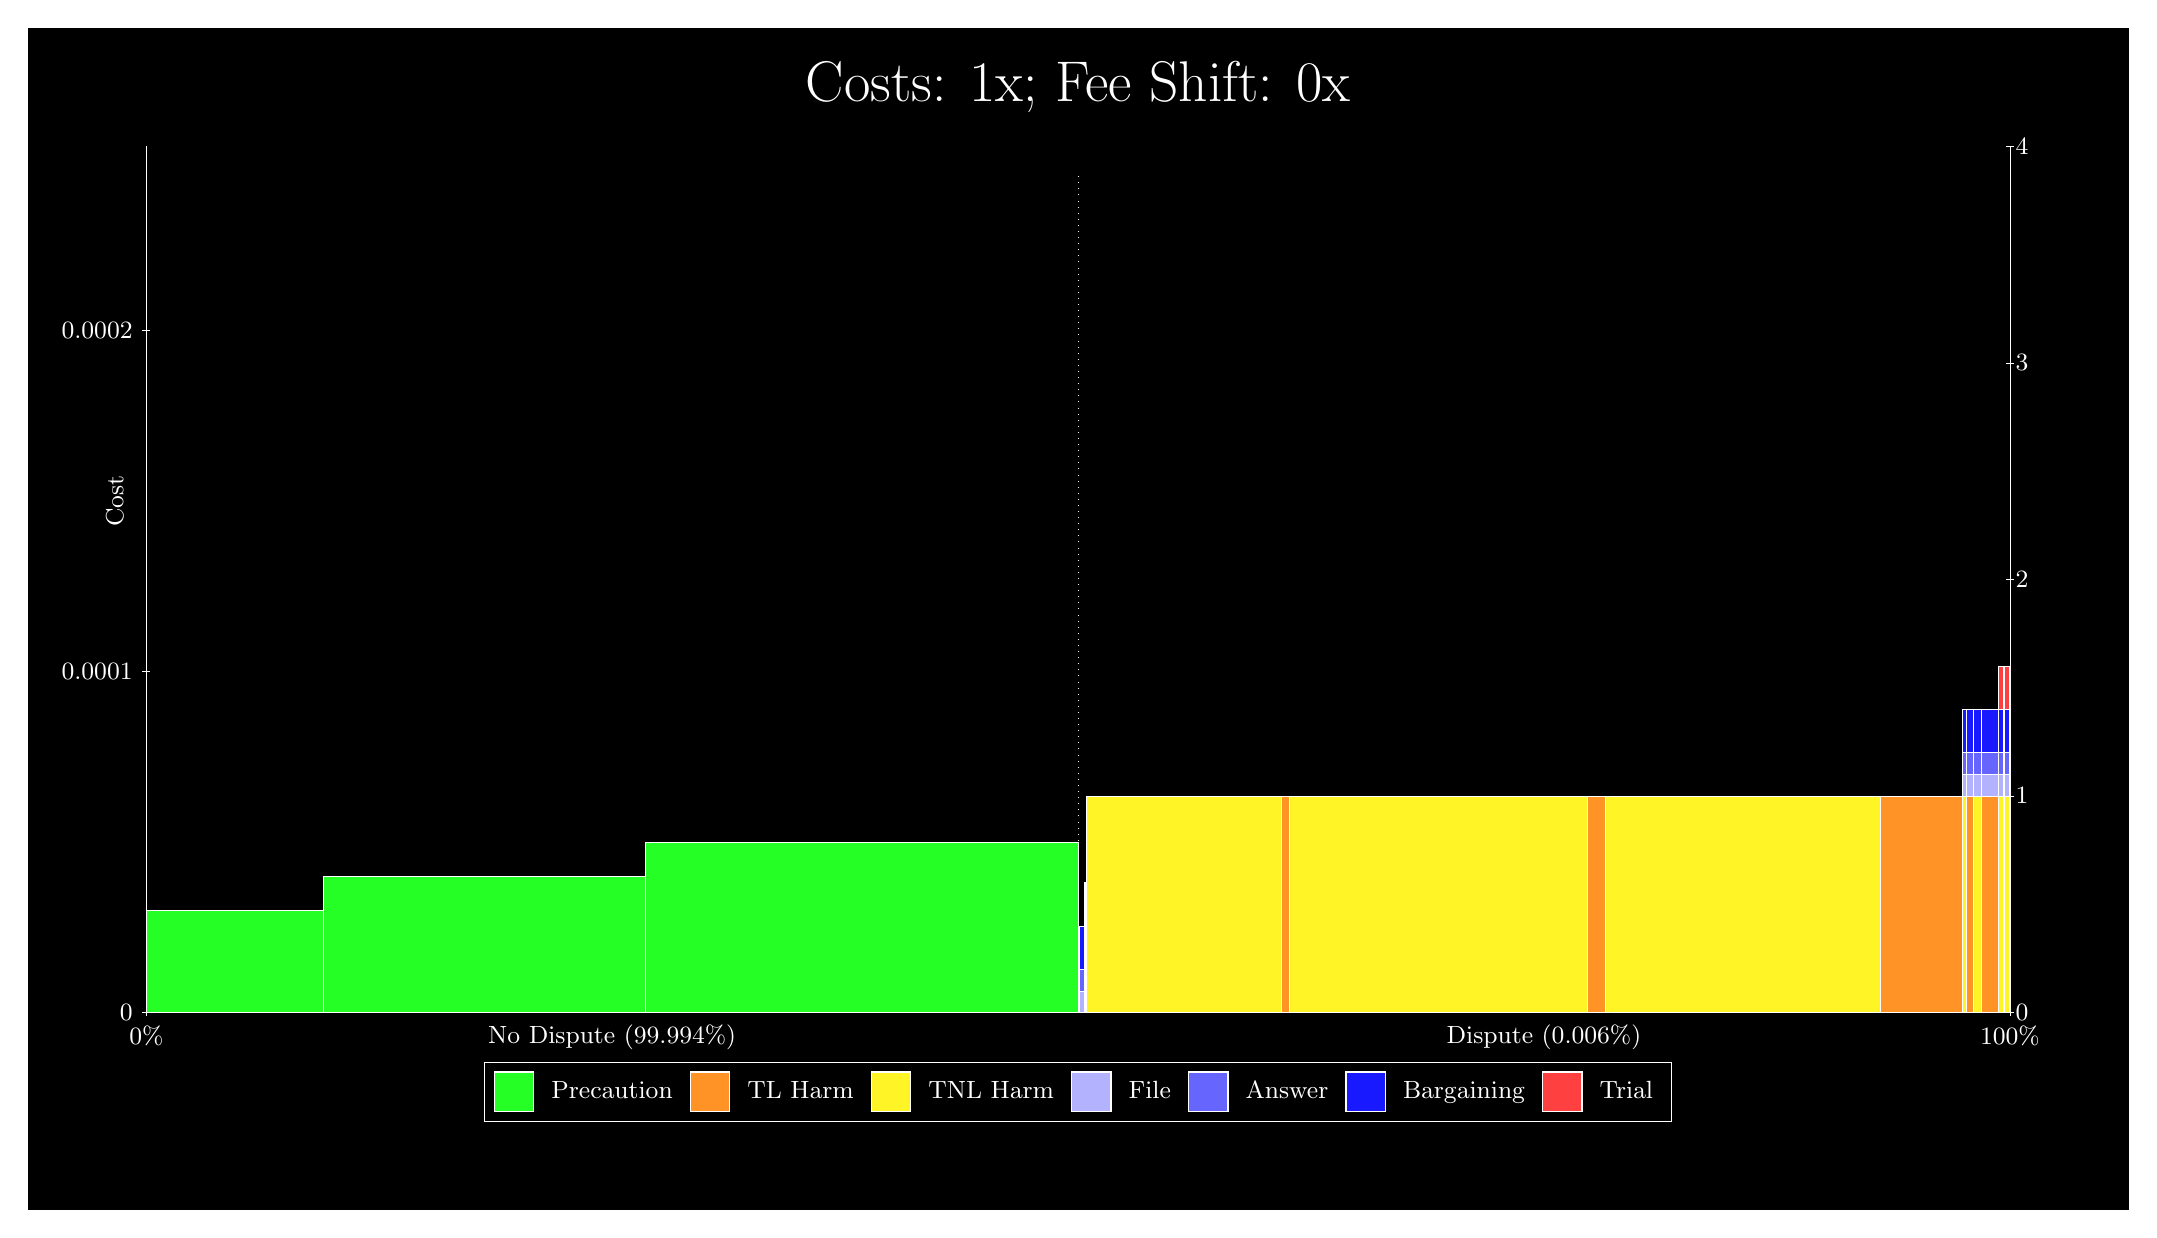
\begin{tikzpicture}
\draw[fill=black] (0,0) rectangle (26.667,15);
\draw[draw=none,text=white] (0,13.5) rectangle (26.667,15) node[midway] {\huge Costs: 1x; Fee Shift: 0x };
\draw[fill=green!85,draw=white,very thin] (1.5,2.5) rectangle (3.7466,3.7993);
\draw[fill=green!85,draw=white,very thin] (3.7466,2.5) rectangle (7.8387,4.2325);
\draw[fill=green!85,draw=white,very thin] (7.8387,2.5) rectangle (13.333,4.6656);
\draw[fill=green!85,draw=white,very thin] (13.333,2.5) rectangle (13.353,2.5001);
\draw[fill=blue!30,draw=white,very thin] (13.333,2.5001) rectangle (13.353,2.7751);
\draw[fill=blue!60,draw=white,very thin] (13.333,2.7751) rectangle (13.353,3.0501);
\draw[fill=blue!90,draw=white,very thin] (13.333,3.0501) rectangle (13.353,3.6001);
\draw[fill=green!85,draw=white,very thin] (13.353,2.5) rectangle (13.409,2.5001);
\draw[fill=blue!30,draw=white,very thin] (13.353,2.5001) rectangle (13.409,2.7751);
\draw[fill=blue!60,draw=white,very thin] (13.353,2.7751) rectangle (13.409,3.0501);
\draw[fill=blue!90,draw=white,very thin] (13.353,3.0501) rectangle (13.409,3.6001);
\draw[fill=green!85,draw=white,very thin] (13.409,2.5) rectangle (13.421,2.5001);
\draw[fill=blue!30,draw=white,very thin] (13.409,2.5001) rectangle (13.421,2.7751);
\draw[fill=blue!60,draw=white,very thin] (13.409,2.7751) rectangle (13.421,3.0501);
\draw[fill=blue!90,draw=white,very thin] (13.409,3.0501) rectangle (13.421,3.6001);
\draw[fill=red!75,draw=white,very thin] (13.409,3.6001) rectangle (13.421,4.1501);
\draw[fill=green!85,draw=white,very thin] (13.421,2.5) rectangle (13.432,2.5001);
\draw[fill=blue!30,draw=white,very thin] (13.421,2.5001) rectangle (13.432,2.7751);
\draw[fill=blue!60,draw=white,very thin] (13.421,2.7751) rectangle (13.432,3.0501);
\draw[fill=blue!90,draw=white,very thin] (13.421,3.0501) rectangle (13.432,3.6001);
\draw[fill=red!75,draw=white,very thin] (13.421,3.6001) rectangle (13.432,4.1501);
\draw[fill=green!85,draw=white,very thin] (13.432,2.5) rectangle (15.918,2.5001);
\draw[fill=yellow!85,draw=white,very thin] (13.432,2.5001) rectangle (15.918,5.2501);
\draw[fill=green!85,draw=white,very thin] (15.918,2.5) rectangle (16.009,2.5001);
\draw[fill=orange!85,draw=white,very thin] (15.918,2.5001) rectangle (16.009,5.2501);
\draw[fill=green!85,draw=white,very thin] (16.009,2.5) rectangle (19.796,2.5001);
\draw[fill=yellow!85,draw=white,very thin] (16.009,2.5001) rectangle (19.796,5.2501);
\draw[fill=green!85,draw=white,very thin] (19.796,2.5) rectangle (20.031,2.5001);
\draw[fill=orange!85,draw=white,very thin] (19.796,2.5001) rectangle (20.031,5.2501);
\draw[fill=green!85,draw=white,very thin] (20.031,2.5) rectangle (23.518,2.5001);
\draw[fill=yellow!85,draw=white,very thin] (20.031,2.5001) rectangle (23.518,5.2501);
\draw[fill=green!85,draw=white,very thin] (23.518,2.5) rectangle (24.558,2.5001);
\draw[fill=orange!85,draw=white,very thin] (23.518,2.5001) rectangle (24.558,5.2501);
\draw[fill=green!85,draw=white,very thin] (24.558,2.5) rectangle (24.618,2.5001);
\draw[fill=yellow!85,draw=white,very thin] (24.558,2.5001) rectangle (24.618,5.2501);
\draw[fill=blue!30,draw=white,very thin] (24.558,5.2501) rectangle (24.618,5.5251);
\draw[fill=blue!60,draw=white,very thin] (24.558,5.5251) rectangle (24.618,5.8001);
\draw[fill=blue!90,draw=white,very thin] (24.558,5.8001) rectangle (24.618,6.3501);
\draw[fill=green!85,draw=white,very thin] (24.618,2.5) rectangle (24.698,2.5001);
\draw[fill=orange!85,draw=white,very thin] (24.618,2.5001) rectangle (24.698,5.2501);
\draw[fill=blue!30,draw=white,very thin] (24.618,5.2501) rectangle (24.698,5.5251);
\draw[fill=blue!60,draw=white,very thin] (24.618,5.5251) rectangle (24.698,5.8001);
\draw[fill=blue!90,draw=white,very thin] (24.618,5.8001) rectangle (24.698,6.3501);
\draw[fill=green!85,draw=white,very thin] (24.698,2.5) rectangle (24.803,2.5001);
\draw[fill=yellow!85,draw=white,very thin] (24.698,2.5001) rectangle (24.803,5.2501);
\draw[fill=blue!30,draw=white,very thin] (24.698,5.2501) rectangle (24.803,5.5251);
\draw[fill=blue!60,draw=white,very thin] (24.698,5.5251) rectangle (24.803,5.8001);
\draw[fill=blue!90,draw=white,very thin] (24.698,5.8001) rectangle (24.803,6.3501);
\draw[fill=green!85,draw=white,very thin] (24.803,2.5) rectangle (25.014,2.5001);
\draw[fill=orange!85,draw=white,very thin] (24.803,2.5001) rectangle (25.014,5.2501);
\draw[fill=blue!30,draw=white,very thin] (24.803,5.2501) rectangle (25.014,5.5251);
\draw[fill=blue!60,draw=white,very thin] (24.803,5.5251) rectangle (25.014,5.8001);
\draw[fill=blue!90,draw=white,very thin] (24.803,5.8001) rectangle (25.014,6.3501);
\draw[fill=green!85,draw=white,very thin] (25.014,2.5) rectangle (25.079,2.5001);
\draw[fill=yellow!85,draw=white,very thin] (25.014,2.5001) rectangle (25.079,5.2501);
\draw[fill=blue!30,draw=white,very thin] (25.014,5.2501) rectangle (25.079,5.5251);
\draw[fill=blue!60,draw=white,very thin] (25.014,5.5251) rectangle (25.079,5.8001);
\draw[fill=blue!90,draw=white,very thin] (25.014,5.8001) rectangle (25.079,6.3501);
\draw[fill=red!75,draw=white,very thin] (25.014,6.3501) rectangle (25.079,6.9001);
\draw[fill=green!85,draw=white,very thin] (25.079,2.5) rectangle (25.101,2.5001);
\draw[fill=orange!85,draw=white,very thin] (25.079,2.5001) rectangle (25.101,5.2501);
\draw[fill=blue!30,draw=white,very thin] (25.079,5.2501) rectangle (25.101,5.5251);
\draw[fill=blue!60,draw=white,very thin] (25.079,5.5251) rectangle (25.101,5.8001);
\draw[fill=blue!90,draw=white,very thin] (25.079,5.8001) rectangle (25.101,6.3501);
\draw[fill=red!75,draw=white,very thin] (25.079,6.3501) rectangle (25.101,6.9001);
\draw[fill=green!85,draw=white,very thin] (25.101,2.5) rectangle (25.154,2.5001);
\draw[fill=yellow!85,draw=white,very thin] (25.101,2.5001) rectangle (25.154,5.2501);
\draw[fill=blue!30,draw=white,very thin] (25.101,5.2501) rectangle (25.154,5.5251);
\draw[fill=blue!60,draw=white,very thin] (25.101,5.5251) rectangle (25.154,5.8001);
\draw[fill=blue!90,draw=white,very thin] (25.101,5.8001) rectangle (25.154,6.3501);
\draw[fill=red!75,draw=white,very thin] (25.101,6.3501) rectangle (25.154,6.9001);
\draw[fill=green!85,draw=white,very thin] (25.154,2.5) rectangle (25.167,2.5001);
\draw[fill=orange!85,draw=white,very thin] (25.154,2.5001) rectangle (25.167,5.2501);
\draw[fill=blue!30,draw=white,very thin] (25.154,5.2501) rectangle (25.167,5.5251);
\draw[fill=blue!60,draw=white,very thin] (25.154,5.5251) rectangle (25.167,5.8001);
\draw[fill=blue!90,draw=white,very thin] (25.154,5.8001) rectangle (25.167,6.3501);
\draw[fill=red!75,draw=white,very thin] (25.154,6.3501) rectangle (25.167,6.9001);
\draw[white,very thin] (1.5,2.5) -- (1.5,13.5);
\node[font=\small,rotate=90,text=white, anchor=center] at (1.1, 8.9967) {Cost};
\draw[white,very thin] (1.45,2.5) -- (1.55,2.5);
\node[font=\small,text=white, anchor=east] at (1.45, 2.5) {0};
\draw[white,very thin] (1.45,6.8311) -- (1.55,6.8311);
\node[font=\small,text=white, anchor=east] at (1.45, 6.8311) {0.0001};
\draw[white,very thin] (1.45,11.162) -- (1.55,11.162);
\node[font=\small,text=white, anchor=east] at (1.45, 11.162) {0.0002};

\draw[white,dotted,very thin] (13.333,2.83) -- (13.333,13.17);
\draw[white,very thin] (25.167,2.5) -- (25.167,13.5);
\draw[white,very thin] (25.117,2.5) -- (25.217,2.5);
\node[font=\small,text=white, anchor=west] at (25.117, 2.5) {0};
\draw[white,very thin] (25.117,5.25) -- (25.217,5.25);
\node[font=\small,text=white, anchor=west] at (25.117, 5.25) {1};
\draw[white,very thin] (25.117,8) -- (25.217,8);
\node[font=\small,text=white, anchor=west] at (25.117, 8) {2};
\draw[white,very thin] (25.117,10.75) -- (25.217,10.75);
\node[font=\small,text=white, anchor=west] at (25.117, 10.75) {3};
\draw[white,very thin] (25.117,13.5) -- (25.217,13.5);
\node[font=\small,text=white, anchor=west] at (25.117, 13.5) {4};

\draw[white,very thin] (1.5,2.5) -- (25.167,2.5);
\draw[white,very thin] (1.5,2.45) -- (1.5,2.55);
\node[font=\small,text=white, anchor=north] at (1.5, 2.45) {0\%};
\draw[white,very thin] (25.167,2.45) -- (25.167,2.55);
\node[font=\small,text=white, anchor=north] at (25.167, 2.45) {100\%};

\node[font=\small,text=white,anchor=south] at (7.4167, 1.9) {No\ Dispute\ (99.994\%)};
\node[font=\small,text=white,anchor=south] at (19.25, 1.9) {Dispute\ (0.006\%)};
\draw (13.3333,2.5) node (B) {};
\begin{scope}[align=center]
\matrix[scale=0.5,draw=white,below=0.5cm of B,nodes={draw},column sep=0.1cm]{
\node[rectangle,draw,minimum width=0.5cm,minimum height=0.5cm,fill=green!85]{}; & \node[draw=none,font=\small,text=white]{Precaution}; &
\node[rectangle,draw,minimum width=0.5cm,minimum height=0.5cm,fill=orange!85]{}; & \node[draw=none,font=\small,text=white]{TL Harm}; &
\node[rectangle,draw,minimum width=0.5cm,minimum height=0.5cm,fill=yellow!85]{}; & \node[draw=none,font=\small,text=white]{TNL Harm}; &
\node[rectangle,draw,minimum width=0.5cm,minimum height=0.5cm,fill=blue!30]{}; & \node[draw=none,font=\small,text=white]{File}; &
\node[rectangle,draw,minimum width=0.5cm,minimum height=0.5cm,fill=blue!60]{}; & \node[draw=none,font=\small,text=white]{Answer}; &
\node[rectangle,draw,minimum width=0.5cm,minimum height=0.5cm,fill=blue!90]{}; & \node[draw=none,font=\small,text=white]{Bargaining}; &
\node[rectangle,draw,minimum width=0.5cm,minimum height=0.5cm,fill=red!75]{}; & \node[draw=none,font=\small,text=white]{Trial}; \\\\
};\end{scope}

\end{tikzpicture}
\end{document}